\documentclass[a4paper]{article}
\usepackage[utf8x]{inputenc}
\usepackage[french]{babel}
\usepackage[T1]{fontenc}

\usepackage[a4paper,top=3cm,bottom=2cm,left=3cm,right=3cm,marginparwidth=1.75cm]{geometry}

\usepackage{amsmath}
\usepackage{graphicx}
\usepackage[colorinlistoftodos]{todonotes}
\usepackage[colorlinks=true, allcolors=blue]{hyperref}

\usepackage{listings}
\usepackage{color}

\definecolor{dkgreen}{rgb}{0,0.6,0}
\definecolor{gray}{rgb}{0.5,0.5,0.5}
\definecolor{mauve}{rgb}{0.58,0,0.82}

\lstset{frame=tb,
  language=Java,
  aboveskip=3mm,
  belowskip=3mm,
  showstringspaces=false,
  columns=flexible,
  basicstyle={\small\ttfamily},
  numbers=none,
  numberstyle=\tiny\color{gray},
  keywordstyle=\color{blue},
  commentstyle=\color{dkgreen},
  stringstyle=\color{mauve},
  breaklines=true,
  breakatwhitespace=true,
  tabsize=3
}

\title{Développement Mobile}
\author{Loïc Dennemont}
\begin{document}
\maketitle

\begin{abstract}
Voici le Rapport du CCTP de développement mobile.
\end{abstract}

\section{Introduction}
Dans le cadre de l'UE de développement mobile, les étudiants sont mené a réalisé un jeu mobile sur les plate forme Android et IOS. Le choix du jeu était libre mais il ne faillait qu'il ne soit pas trop simple. De plus, il faillait que le jeu intègre un score a chaque partie, une persistance des données, une présentation sous forme de liste et pouvoir fonctionner sur tout type d'écran.J'ai choisi de réaliser un casse brique.
\subsection{Description de l'application}
L'application développé dans le cadre de l'UE est un casse brique. C'est un jeu qui consiste a détruite une série de brique en haut de l'écran a l'aide d'une raquette contrôlé par le joueur en bas de l'écran. Quand le jeu commence, une balle tombe sur la raquette, et rebondit sur elle et les murs. Si la balle touche une brique, elle la détruit et rebondit, faisant gagné au joueur des points. Quand la balle touche le bas de l'écran, il perd une vie A zéro, il perd la partie.

\section{Android} 
\subsection{Structure général}
Pour l'application Android, l'application et composé de quatre parties:
\subparagraph{-Menu principal}
Quand le joueur démarre l'application, il se retrouve sur cette View.Elle possède deux boutons et une zone ou l'utilisateur peut rentrer son nom. Le premier bouton est le bouton "START" qui permet de lancer le jeu. Le deuxième est le bouton "RESULT" qui permet de visualisé les 3 meilleurs scores.
\subparagraph{-Jeu} Voici la partie principal de l'application. C'est ici que l'utilisateur va joueur au jeu. Sur cette écran, on peut apercevoir en haut a gauche le score et la vie restant.En haut a droite se trouve un bouton pause qui permet mettre en pause et d'afficher des options. Enfin, on peut voir au centre la balle et en bas la raquette. Un message invite a toucher l'écran pour commencer la partie. En touchant l'écran, les briques apparaîtrons sur l'écran.\\
Quand on appuis sur le boutons pauses, 3 boutons apparaissent. Deux boutons en bas pour activer ou désactiver le son du jeu et la vibration. Et un au centre pour quitter la partie en cours.

Cette classe génère les briques et gère la partie( le déplacement de la balle, les collision, les événements, etc...).

\subparagraph{-Game Over} Quand le joueur perd la partie, il arrive ici. Cette View est composé d'un texte de "GAME OVER", le nom de l'utilisateur et son score, d'un bouton pour recommencer et un autre pour quitter le jeu et du meilleur score réalisé. \\
Si l'utilisateur réalise un meilleur score, il remplace celui existant et décale les autres d'une place inférieur (Celle le meilleur score est afficher sur cette écran). Pour indiquer au joueur qu'il a fait le meilleur score, le texte s'affiche en rouge.
\pagebreak

\subparagraph{-Résultat} La dernière View de l'application, elle affiche les 3 meilleurs score réalisé sur l'appareil. Elle a aussi un bouton permettant de revenir au menu principal.


\subsection{Quelque point}
\subparagraph{Moteur physique} Android Studio ne possède pas de moteur physique. J'ai du codé moi même la physique de la balle et les collisions entre les différents objets (La balle, la raquette, les briques et les murs). Pour simplifier la collision, j'ai utilisé une balle carré car il était plus facile de détecter une collision en deux rectangles qu'avec un cercle et un rectangle.
\subparagraph{Collision} Pour gérer la collision entre les éléments du jeu, j'utilise une classe collision, qui a pour paramètre deux rectangles, qui sont les "hitbox" des deux éléments.
\begin{lstlisting}
    public boolean collision(rectangle a ,rectangle b){
        return (((b.x1-a.x2)*(b.x2-a.x1)<=0) && ((b.y1-a.y2)*(b.y2-a.y1)<=0));
    }
\end{lstlisting}
\subparagraph{Rotation de l'écran} Pour cette application, la rotation de l'écran est bloqué en mode portrait pour évite des problème déformation du terrain de jeu. En effet, comme la hauteur et la largeur ont une taille différente.\\ Si on tourne l'écran, soit les éléments seront étirer, soit l'espace entre les briques et la raquette changerai,soit la difficulté du jeu serait modifié.
\subparagraph{Persistance des données} Pour enregistrer les scores, l'application utilise la méthode "SharedPreferences".
\subparagraph{Victoire}Il n'y a pas de victoire dans se jeu. En effet, quand toute les briques ont été détruit, le jeu recommence mais garde le score précédant.
\subparagraph{Amélioration}Ceci est la première version du casse brique et si j'avais plus de temps, plusieurs amélioration peuvent possible pour avoir un meilleur jeu comme l'ajout de bonus ou une difficulté croissante ( balle qui augmente sa vitesse a chaque niveau).
\subsection{Image de l'application}
\begin{center}
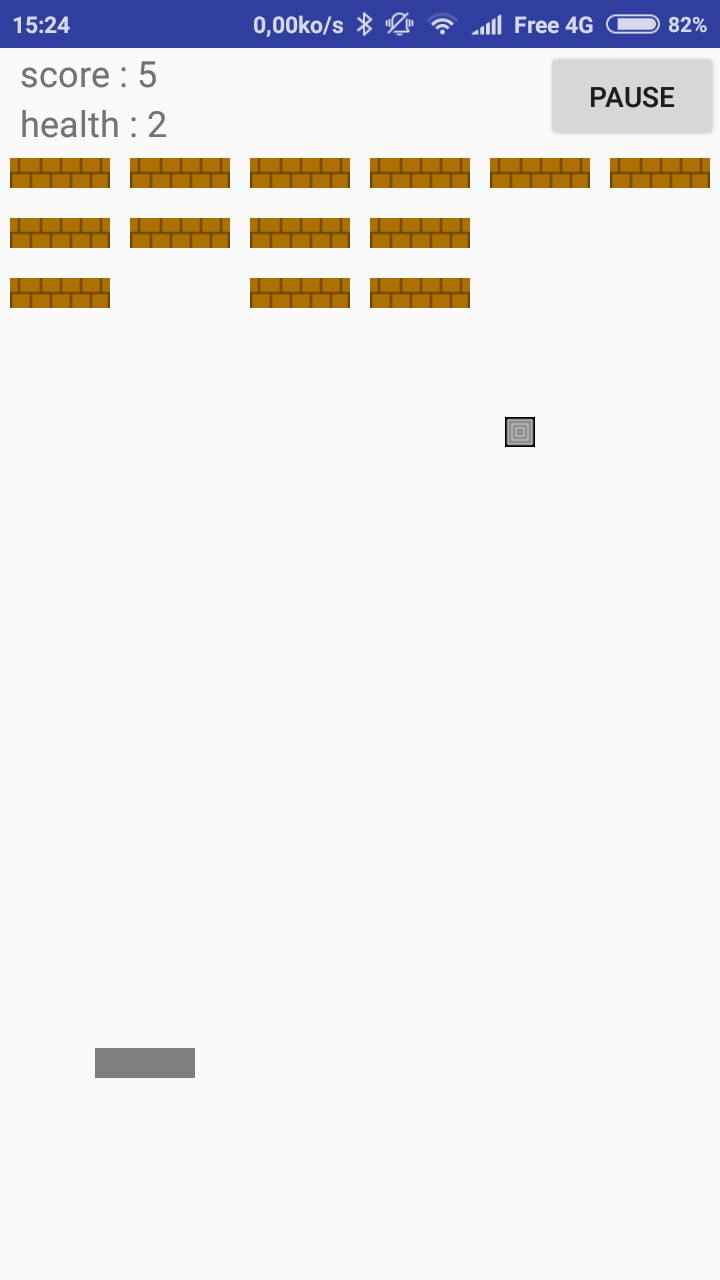
\includegraphics[scale=0.25]{android.png}
\end{center}
\pagebreak

\section{IOS}
\subsection{Structure général}
Pour l'application IOS, elle est composé 2 classes:
\subparagraph{ViewController}C'est la première classe de l'application. Ça fonction est de charger la classe raquette et de mettre a jour le texte a l'écran.
\subparagraph{Raquette} C'est la classe principal de l'application. C'est elle qui gère tous le jeu, de la génération de brique au contrôle de la raquette en passant par le déplacement de la balle. Elle affiche le message "Game Over" et de Victoire.
\subsection{Quelque point}
\subparagraph{Difficulté de développement}
Contrairement a Android, la conception d'application est plus compliqué. En effet, pour pouvoir programmer sur IOS, il faut posséder un mac, qui est plus onéreux qu'un pc classique et pas forcement accessible pour un étudiant. N'ayant pas de mac, je me suis tourné sur une machine virtuelle. Malheureusement, le manque de puissance de mon ordinateur m’empêchais de programmer de façon fluide. Finalement, j'ai réaliser la partie IOS au PTU avec des contrainte de temps et de déplacement.
\subsection{Image de l'application}
\begin{center}
 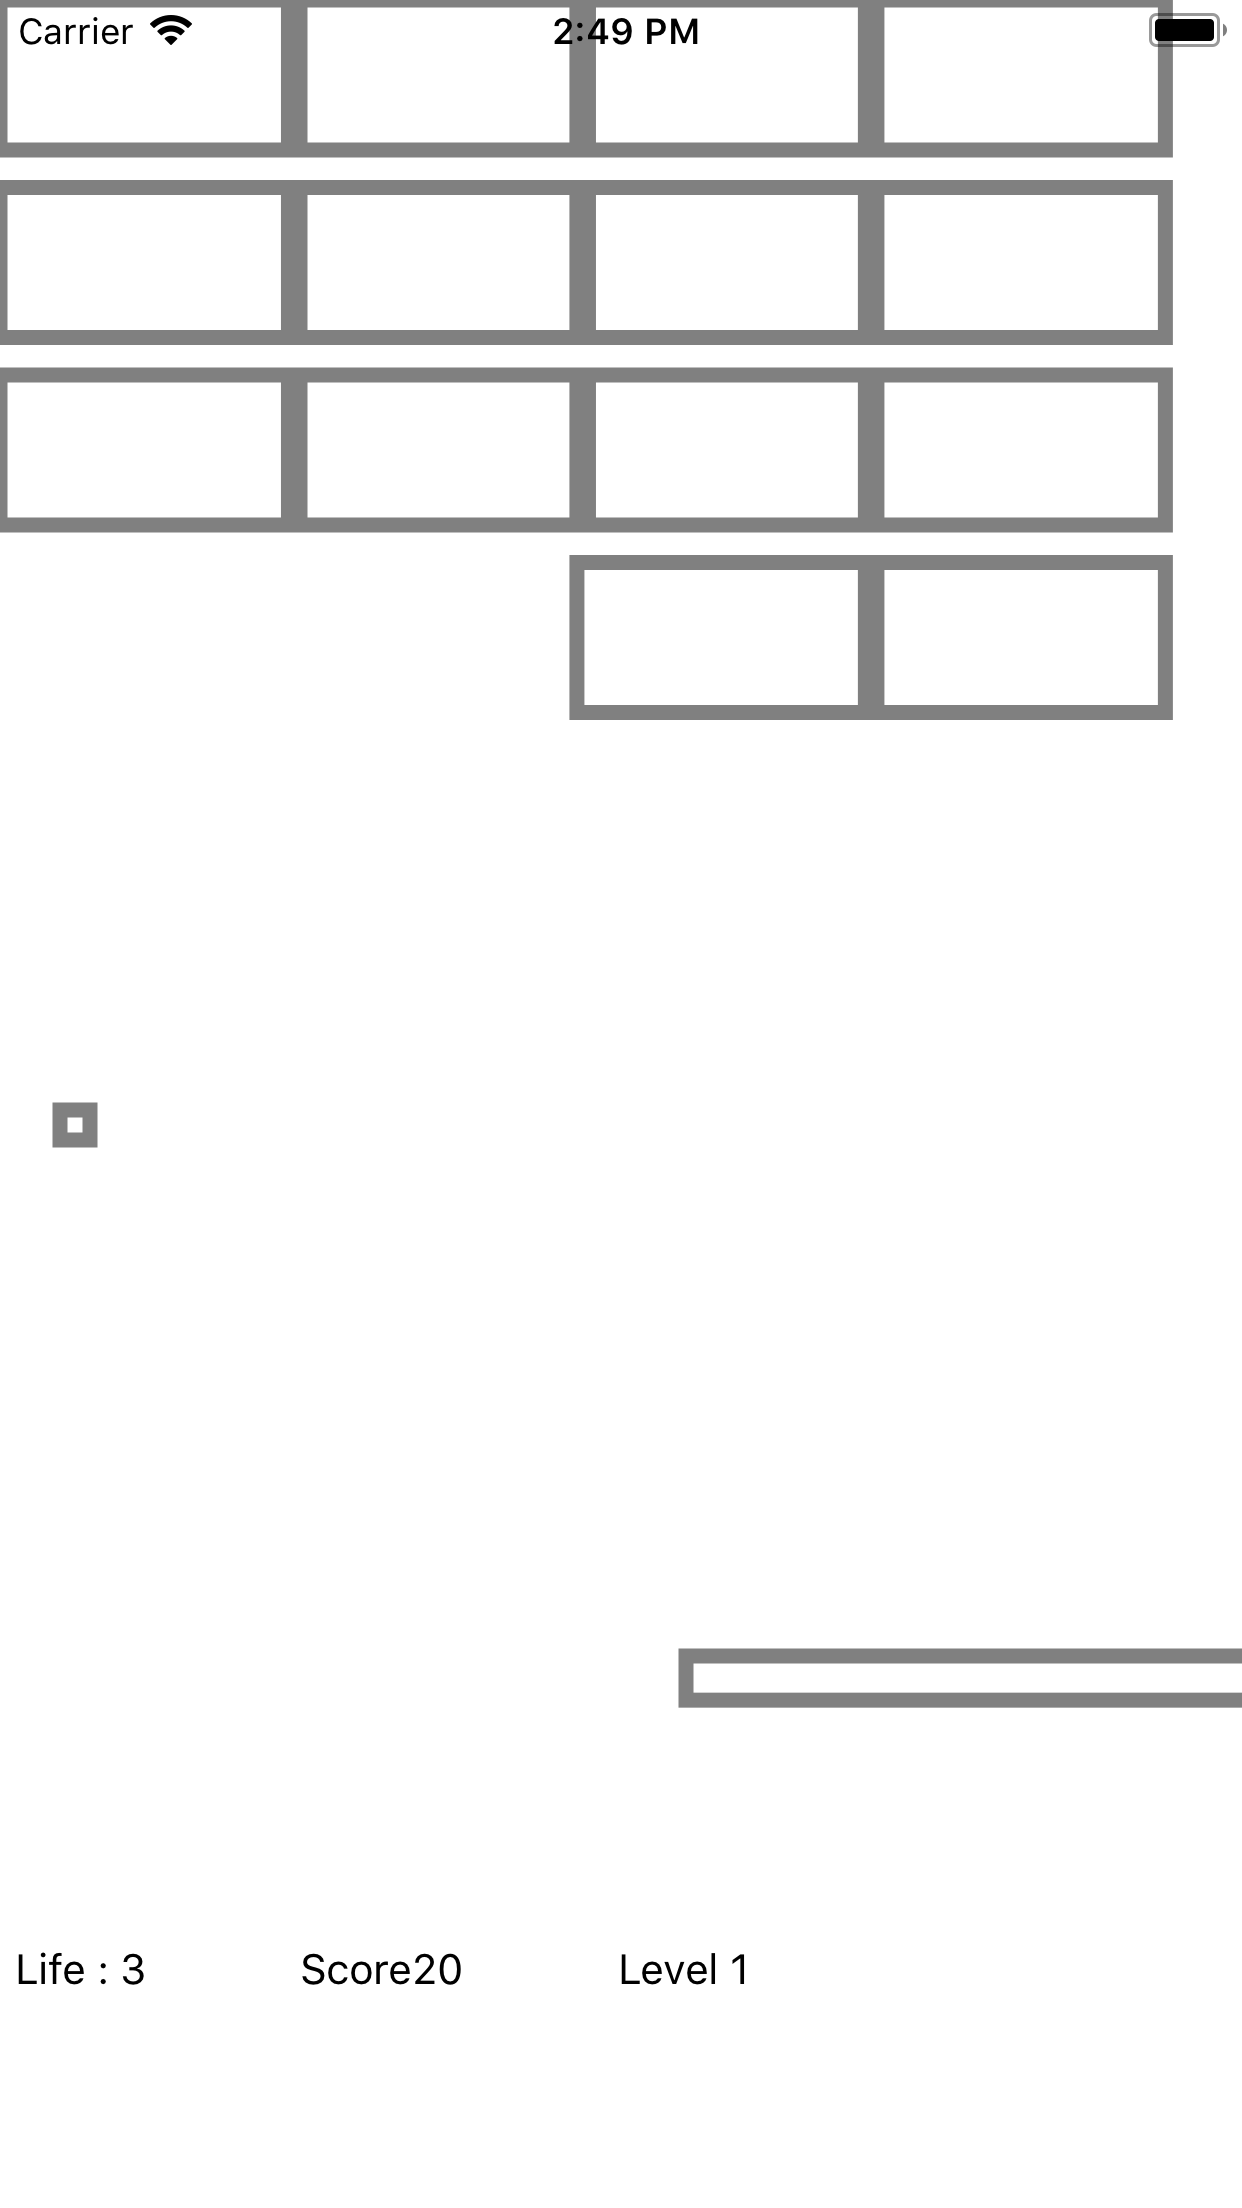
\includegraphics[scale=0.25]{IOS.png}
\end{center}
\section{Conclusion}
Cette UE de développement mobile m'a appris les enjeux de développer des applications sur Android et IOS. Elle m'a permit d’appréhender les difficulté comme prendre en compte toutes les tailles d'écrans dans le design.
\end{document}
